The phase field method, rooted in system thermodynamics, offers a solution for an interface with a finite thickness, an idea originating from van der Waals in 1893 \cite{vanderwaals1979ThermodynamicTheoryCapillarity}. This method models the free energy of the system and can derive a phase field method for interfacial dynamics. It offers several advantages, such as mass conservation, contact line motion, and adherence to thermodynamic laws. In contrast to the hydrodynamic theory, the contact line moves through interfacial diffusion. However, there are concerns about its validity in modeling macroscopic contact line motion, especially regarding the sharp-interface limit. Despite these concerns, meaningful results have been predicted on the macro scale that align with hydrodynamic theory and experimental observations\cite{yue2010SharpinterfaceLimitCahn,yue2011CanDiffuseinterfaceModels,carlson2011DissipationRapidDynamic}.


Phase field simulations for macroscopic wetting typically rely on the Cahn-Hilliard equations. For slow wetting phenomena, the phase field theory has been both analytically \cite{jacqmin2000ContactlineDynamicsDiffuse} and numerically \cite{yue2011CanDiffuseinterfaceModels,yue2010SharpinterfaceLimitCahn} proven to capture such wetting physics. However, for rapid spreading of water drops, the assumption of local equilibrium may not hold. Some studies have introduced a boundary condition for wetting far from equilibrium, introducing a parameter that controls the relaxation towards equilibrium . This parameter has been interpreted in various ways, from a local friction adjacent to the contact line to a relaxation parameter at the contact line\cite{yue2011WallEnergyRelaxation}\cite{carlsonCapillarityDynamicWetting2012}.


\todo[inline]{einleitende Worte}

Wie bereits in Kapitel \ref{sec: Wetting_SurfaceTension} beshcrieben, gibt es unterschiedliche Möglichkeiten das Interface zu beschreiben. Hydrodynamische Modelle beschreiben das Interface so, dass am Übergang der Phasen die Stoffwerte springen. Ein Diffuses Interface hingegen, beschreibt die größen anders. \todo{picture of interfaces}

\section{Phase Field Method in the Spirit of Cahn and Hillard}
The phase field method traces back to the idea of van der Waals \cite{vanderwaals1979ThermodynamicTheoryCapillarity}, who described the interface between two immiscible fluids from a thermodynamic perspective. In this description, the material properties transition continuously within a thin layer. Within this layer, both phases coexist.

Building on this, Cahn and Hillard \cite{johnw.FreeEnergyNonuniform1958} derived a description of the free energy in a volume with non-uniform composition as a function of an order parameter $C$ for time-dependent problems. In its closed form, it reads
\begin{equation}
\label{eq: CahnHillard}
    \partial C + \textbf{u} \cdot \nabla C = \nabla \cdot \left(\kappa \nabla \phi(C)\right).
\end{equation}
Here, $\textbf{u}$ is the velocity, $\kappa$ is a diffusion coefficient, often referred to as mobility, and $\phi$ is a chemical potential. The order parameter indicates which phase is present and ranges between $-1$ and $1$ for a two-phase system. The mobility can be related to the Péclet number, which represents the ratio of advective to diffusive fluxes with a characteristic path length ($L_{char}$) and velocity ($u_{char}$), as well as a characteristic chemical potential \cite{cai2015NumericalSimulationWetting,holzinger2021DirectNumericalSimulation}.

The chemical potential is defined as the derivative of the Helmholtz free energy with respect to the order parameter \cite{johnw.FreeEnergyNonuniform1958}. In the system under consideration, the total free energy consists of the mixing energy and the interfacial density energy. According to \cite{yue2010SharpinterfaceLimitCahn}, the system's free energy is influenced by two factors; defined over the volume $\Omega$ and the surface $\partial\Omega$ \todo{check!!!}
\begin{equation}
    F(C, \nabla C) = \int_{\Omega} f_{\mathrm{mix}} (C, \nabla C) d\textbf{x}+ \int_{\partial\Omega}f_\mathrm{w}(C) dS
\end{equation}
Here, the first integral represents the mixing energy density $f_{mix}$, and the second represents the wall energy $f_w$.


\subsection{Mixing Energy}
Cahn and Hillard defined a mixing energy ($f_{\text{mix}}$) that depends on the order parameter and its gradient:
\begin{equation}
    F(C, \nabla C) = \int_{\Omega} f_{\mathrm{mix}} (C, \nabla C) d\textbf{x} = \int_{\Omega}\left(\frac{\lambda}{\epsilon^2}\Psi(C)+\frac{\lambda}{2}\vert\nabla C\vert^2\right)d\textbf{x}
\end{equation}\todo{check if right function}
The integration of the mixing energy over the domain yields the Helmholtz free energy of the fluid system and consists of two terms. The first term separates the phases from each other, while the second term mixes the phases. $\lambda$ is a mixing energy parameter, $\epsilon$ a measure for the thickness of the interface\todo{check if already mentioned}, and $\Psi$ a potential. The potential is chosen according to Ginzburg and Landau\todo{cite} so that it has two minima at positions $-1$ and $1$ and is given by 
\begin{equation}
    \Psi(C)= \frac{1}{4}\left(C^2-1\right)^2.
\end{equation}
This leads to the following representation for the chemical potential 
\begin{equation}
    \label{eq: chempotentialMIXING_pahseFieldMethod}
    \Phi(C):= \frac{\partial F(C)}{\partial C} = \frac{\lambda}{\epsilon^2}\Psi'(C)-\lambda\nabla^2C.
\end{equation}

\subsection{Diffusive Interface}
The Cahn-Hillard model can describe systems with multiple fluids. However, only a binary fluid system is considered in this work.
\begin{figure}[h]
    \centering
    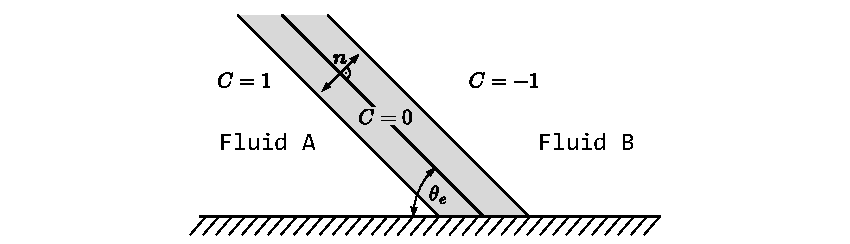
\includegraphics[width=.95\textwidth]{Pictures/DiffusiveInterface.pdf}
    \caption{Schematic representation of a diffusive interface}
    \label{fig: DiffusiveInteraface}
\end{figure}
Figure \ref{fig: DiffusiveInteraface} shows the contact line of a diffusive interface. The gray area is the transition area of the order parameter and thus the material quantities. Within this area, both fluids coexist with their respective densities and viscosities. In the equilibrium state, the profile of $C$ normal to the interface can be determined by minimizing the free energy (Equation \ref{eq: chempotentialMIXING_pahseFieldMethod}) \cite{cai2015NumericalSimulationWetting}. This then leads to a description of the order parameter normal to the interface with
\begin{equation}
    \label{eq: InterfactialNormalDirProfile}
    C(n) = \tanh\left(\frac{n}{\sqrt{2}\epsilon}\right).
\end{equation}
Here, $n$ is the normal to the interface. In equilibrium, the thickness of the diffuse interface remains constant in a range of $3/\sqrt{2}\epsilon$ and for the order parameter $-0.9\leq C\leq0.9$. Also in the case of equilibrium, the surface tension equals the integral of the free energy density at the interface, from which a description for the surface tension can be derived \cite{jacqmin2000ContactlineDynamicsDiffuse}.
\begin{equation}
\label{eq: surfacetensionEqui}
    \sigma = \int_{-\infty}^{\infty}\lambda\left( \frac{dC}{dn}  \right)^{2}= \frac{2\sqrt{2}}{3} \frac{\lambda}{\epsilon}
\end{equation}

\subsection{Wall Energy}
Jaqcmin \cite{jacqmin1999CalculationTwoPhaseNavier} postulated a wall energy of the form
\begin{equation}
    F_{\mathrm{w}}=\int \sigma g(C)dA, 
\end{equation}
where the wall energy is now only a function dependent on the fluid composition directly at the wall. The resulting natural phase field boundary condition with local thermal equilibrium is given by
\begin{equation}
    \label{eq: BCfWall}
    \lambda \frac{\partial C}{\partial n_{\partial \Omega}} + f'_{\mathrm{w}}(C) =0.
\end{equation}
With $n_{\partial \Omega}$ as the normal direction on the wall (cf. \ref{fig: DiffusiveInteraface}).
The normal direction to the interface can be described with the wall normal and wall tangential direction on the wall. 
\begin{equation}
    \label{eq: InterfaceNormal}
    n=n_{\partial\Omega}\cos{(\theta_{\mathrm{e}})}+\tau_{\partial\Omega}\sin{(\theta_{\mathrm{e}})}.
\end{equation}
Subsequently, for the first term from Equation \ref{eq: BCfWall} with Equations \ref{eq: InterfaceNormal}, \ref{eq: InterfactialNormalDirProfile}, and \ref{eq: surfacetensionEqui}, the following can be established
\begin{equation}
    \lambda\frac{\partial C}{\partial n_{\partial\Omega}} =\underbrace{\frac{3}{4}\sigma\left(1-C^2\right)\cos\theta_{\mathrm{e}}}_{=:-f'_\mathrm{w}(C)}.
\end{equation}
From this, a function for the wall energy density can be derived after integration \cite{jacqmin2000ContactlineDynamicsDiffuse}\cite{holzinger2021DirectNumericalSimulation}.
\begin{equation}
    \label{eq: wallfreeenergydensity}
    f_{\mathrm{w}}(C)=-\sigma \cos\theta_{\mathrm{e}} \frac{C(3-C^2)}{4} + \frac{\sigma_{S_L}+ \sigma_{S_V}}{2}
\end{equation}
When only one of the phases is present, this equation only returns the respective surface tension. However, Yue et al. \cite{yue2011WallEnergyRelaxation} point out that this description of wall energy for equilibrium contact angles close to $0^{\circ}$ or $180^{\circ}$ is difficult to reproduce, and the model is not capable of handling precursor films.
With equations \ref{eq: BCfWall} and \ref{eq: wallfreeenergydensity} and the definition of zero flux through the wall, the wetting boundary condition can be described as
\begin{equation}
    \frac{\partial C}{\partial n_{\partial\Omega}} = \frac{\cos \theta_{\mathrm{e}}}{\sqrt{2}\epsilon}(1-C^2).
\end{equation}

\paragraph{Non-Equilibrium Boundary Condition}
\label{sec: nonEquiBC}
Typically, the equilibrium boundary condition (Equation \ref{eq: BCfWall}) is used, neglecting any non-equilibrium effects near the wall. Jacqmin \cite{jacqmin2000ContactlineDynamicsDiffuse} proposed, and Yue et al. \cite{yue2011WallEnergyRelaxation} as well as Qian et al. \cite{qian2006VariationalApproachMoving} studied a generalized version of Equation \ref{eq: BCfWall}.
\begin{equation}
    \frac{\partial C}{\partial t} + \mathbf{u}_{\mathrm{w}}\cdot \nabla C = -\Gamma_{\mathrm{w}} \underbrace{\left(\lambda \frac{\partial C}{\partial n_{\partial \Omega}}+f'_{\mathrm{w}(C)}\right)}_{=:\phi_{\mathrm{w}}}
\end{equation}
Here, $\Gamma_{\mathrm{w}}$ is a newly introduced constant, termed the \textit{wall relaxation parameter}. The wall velocity is represented by $\mathbf{u}_{\mathrm{w}}$. According to Qian et al. \cite{qian2006VariationalApproachMoving}, for $\Gamma_{\mathrm{w}}\rightarrow 0$ and $\kappa\rightarrow 0$, the sharp interface limit with dominant advection is obtained. In the opposite case, diffusion becomes dominant. The wall relaxation parameter serves as an adjustable parameter for the simulation and should be understood as a phenomenological parameter. This parameter depends on both the fluid system and the fluid-wall combination \cite{jacqmin2000ContactlineDynamicsDiffuse}.


\section{Cahn-Hillard Navier Stokes Equations}
The coupled Cahn-Hillard Navier Stokes equations are given by
\begin{align}
    \partial_t C + \nabla \cdot \left( C \mathbf{u} \right) &= -\nabla \cdot \mathbf{J} \\
    \nabla \cdot \mathbf{u} &= 0 \\
    \label{eq: NSEChanged}
    \partial_t(\rho \mathbf{u}) + \nabla \cdot (\rho \mathbf{u}\mathbf{u})&= -\nabla \tilde{p} + \nabla \mathbf{\tau} - \nabla \cdot(\mathbf{u}\mathbf{J})-\phi\nabla C + \mathbf{f}_{\mathrm{b}}
\end{align}

Wherein, $\tilde{p}$ is a modified pressure that arises from the Korteweg tensor to account for capillarity and is defined as
\begin{equation}
    \tilde{p} = p + \frac{f_{\mathrm{mix}}}{2}.
\end{equation}
Assuming a Newtonian fluid, $\mathbf{\tau} = 2\mu \mathrm{dev}\mathbf{D}$ with $\mathbf{D} = 1/2[\nabla \mathbf{u}+(\nabla \mathbf{u})^{\mathrm{T}}]$ as the deformation tensor. Furthermore, the density $\rho$ and viscosity $\mu$ are volumetrically averaged with 
\begin{equation}
    \rho = \frac{1 + C}{2} \rho_1 +\frac{1 + C}{2} \rho_2.
\end{equation} 
Here, the suffixes $1$ and $2$ are markers for the respective phases. The viscosity is calculated analogously. The term $- \nabla \cdot(\mathbf{u}\mathbf{J})$ is necessary to ensure thermal consistency \cite{ding2007DiffuseInterfaceModel}. $\mathbf{J}$ is the phase-field flux and, according to Landau and Lifshitz \todo{cite}, $\mathbf{J} = -\kappa \nabla \phi$ and therefore the phase-field system is driven by the gradient of the local chemical potential. 


